%%%%%%%%%%%%%%%%%%%%%%%%%%%%%%%%%%%%%%%%%
% Beamer Presentation
% LaTeX Template
% Version 1.0 (10/11/12)
%
% This template has been downloaded from:
% http://www.LaTeXTemplates.com
%
% License:
% CC BY-NC-SA 3.0 (http://creativecommons.org/licenses/by-nc-sa/3.0/)
%
%%%%%%%%%%%%%%%%%%%%%%%%%%%%%%%%%%%%%%%%%

%----------------------------------------------------------------------------------------
%	PACKAGES AND THEMES
%----------------------------------------------------------------------------------------

\documentclass[aspectratio=169,usenames,dvipsnames]{beamer}

\usepackage[utf8]{inputenc}
\usepackage{booktabs}
\usepackage{tabularx}
\usepackage{amsmath}
\usepackage[authordate,bibencoding=auto,strict,backend=biber,natbib]{biblatex-chicago}
\addbibresource{bib.bib}
\usepackage{graphicx}
% \hypersetup{
%     colorlinks,
%     %citecolor=black,
%     linkcolor=black
% }
\usepackage{array}
\usepackage{caption}
\usepackage{threeparttable}
\usepackage{epigraph} 
\usepackage{lscape}
\usepackage{adjustbox}
\newcommand*{\Scale}[2][4]{\scalebox{#1}{\ensuremath{#2}}}%
\usepackage{import}
\newenvironment{wideitemize}{\itemize\addtolength{\itemsep}{10pt}}{\enditemize}
\usepackage{amsmath}
\usepackage{csvsimple}
\usepackage{siunitx}
\usepackage{filecontents}
\usepackage{rotating}
\usepackage{multirow}
\usepackage{amsmath}
\usepackage{subcaption}
\usepackage{appendixnumberbeamer}
\usepackage{float}
\usepackage{amsmath}
\usepackage{csvsimple}
\usepackage{hyperref}
\newtheorem{proposition}{Proposition}
\usepackage{xcolor}
\def\boxit#1#2{%
    \smash{\color{red}\fboxrule=1pt\relax\fboxsep=2pt\relax%
    \llap{\rlap{\fbox{\phantom{\rule{#1}{#2}}}}~}}\ignorespaces
}
\newenvironment{variableblock}[3]{%
  \setbeamercolor{block body}{#2}
  \setbeamercolor{block title}{#3}
  \begin{block}{#1}}{\end{block}}
\usepackage{appendixnumberbeamer}
\usepackage{tikz,pgfplots}
\usepackage{tkz-fct}
\usepackage{amsthm}
\pgfplotsset{compat=1.10}
\usepgfplotslibrary{fillbetween}
\mode<presentation> {
\AtBeginSection[]
{
    \begin{frame}
        \frametitle{Table of Contents}
        \tableofcontents[currentsection]
    \end{frame}
}
% The Beamer class comes with a number of default slide themes
% which change the colors and layouts of slides. Below this is a list
% of all the themes, uncomment each in turn to see what they look like.

\usetheme{default}
%\usetheme{AnnArbor}
%\usetheme{Antibes} -
%\usetheme{Bergen}
%\usetheme{Berkeley}
%\usetheme{Berlin}
%\usetheme{Boadilla}
%\usetheme{CambridgeUS}
%\usetheme{Copenhagen} -
%\usetheme{Darmstadt}
%\usetheme{Dresden}
%\usetheme{Frankfurt}
%\usetheme{Goettingen}
%\usetheme{Hannover}
%\usetheme{Ilmenau}
%\usetheme{JuanLesPins}
%\usetheme{Luebeck}
%\usetheme{Madrid}
%\usetheme{Malmoe}
%\usetheme{Marburg}
%\usetheme{Montpellier}
%\usetheme{PaloAlto}
%\usetheme{Pittsburgh}
%\usetheme{Rochester} -
%\usetheme{Singapore}
%\usetheme{Szeged}
%\usetheme{Warsaw}

% As well as themes, the Beamer class has a number of color themes
% for any slide theme. Uncomment each of these in turn to see how it
% changes the colors of your current slide theme.

%\usecolortheme{albatross}
%\usecolortheme{beaver}
%\usecolortheme{beetle}
%\usecolortheme{crane}
%\usecolortheme{dolphin}
%\usecolortheme{dove}
%\usecolortheme{fly}
%\usecolortheme{lily}
%\usecolortheme{orchid}
%\usecolortheme{rose}
%\usecolortheme{seagull}
%\usecolortheme{seahorse}
%\usecolortheme{whale}
%\usecolortheme{wolverine}

%\setbeamertemplate{footline} % To remove the footer line in all slides uncomment this line
%\setbeamertemplate{footline}[frame number] % To replace the footer line in all slides with a simple slide count uncomment this line
\setbeamertemplate{theorems}[numbered]
\setbeamertemplate{navigation symbols}{} % To remove the navigation symbols from the bottom of all slides uncomment this line
}
\setbeamertemplate{caption}{\raggedright\insertcaption\par}
  \setbeamertemplate{enumerate items}[default]
  %\setbeamertemplate{page number in head/foot}{\insertframenumber}
\usepackage{graphicx} % Allows including images
\usepackage{booktabs} % Allows the use of \toprule, \midrule and \bottomrule in tables
%\usepackage {tikz}
\newtheorem*{theorem*}{Theorem}
\newtheorem*{lemma*}{Lemma}
\newtheorem*{proposition*}{Proposition}
\newtheorem*{corollary*}{Corollary}
\newtheorem*{definition*}{Definition}
\DeclareMathOperator*{\argmin}{arg\,min}
\newtheorem*{assumption}{Assumption}
\usetikzlibrary {positioning}
\renewcommand{\arraystretch}{1.5}
\newcommand\hideit[1]{%
  \only<0| handout:1>{\mbox{}}%
  \invisible<0| handout:1>{#1}}
\usepackage[default]{lato}

\setbeamercolor{block body alerted}{bg=alerted text.fg!10}
\setbeamercolor{block title alerted}{bg=alerted text.fg!20}
\setbeamercolor{block body}{bg=structure!10}
\setbeamercolor{block title}{bg=structure!20}
\setbeamercolor{block body example}{bg=green!10}
\setbeamercolor{block title example}{bg=green!20}


\makeatletter
\let\save@measuring@true\measuring@true
\def\measuring@true{%
  \save@measuring@true
  \def\beamer@sortzero##1{\beamer@ifnextcharospec{\beamer@sortzeroread{##1}}{}}%
  \def\beamer@sortzeroread##1<##2>{}%
  \def\beamer@finalnospec{}%
}
\makeatother
%\usepackage {xcolor}

%----------------------------------------------------------------------------------------
%	TITLE PAGE
%----------------------------------------------------------------------------------------

\title[diss]{Lecture 18: Compensation Based on Education} % The short title appears at the bottom of every slide, the full title is only on the title page
\author{Compensation in Organizations} % Your name
\institute[shortinst]{Jacob Kohlhepp}
\date{\today} % Date, can be changed to a custom date

\begin{document}

\begin{frame}
\titlepage % Print the title page as the first slide

\end{frame}


\begin{frame}{Discussion}

\huge From the perspective of a social planner, should people with more education be paid more?
    
\end{frame}


\begin{frame}{Discussion}

\huge From the perspective of an individual organization, should people with more education be paid more?
\end{frame}


\begin{frame}{Discussion - Reading}

\huge Blair and Chung (2022)
\end{frame}


\begin{frame}{Average Salary by Level of Education in the U.S.}

    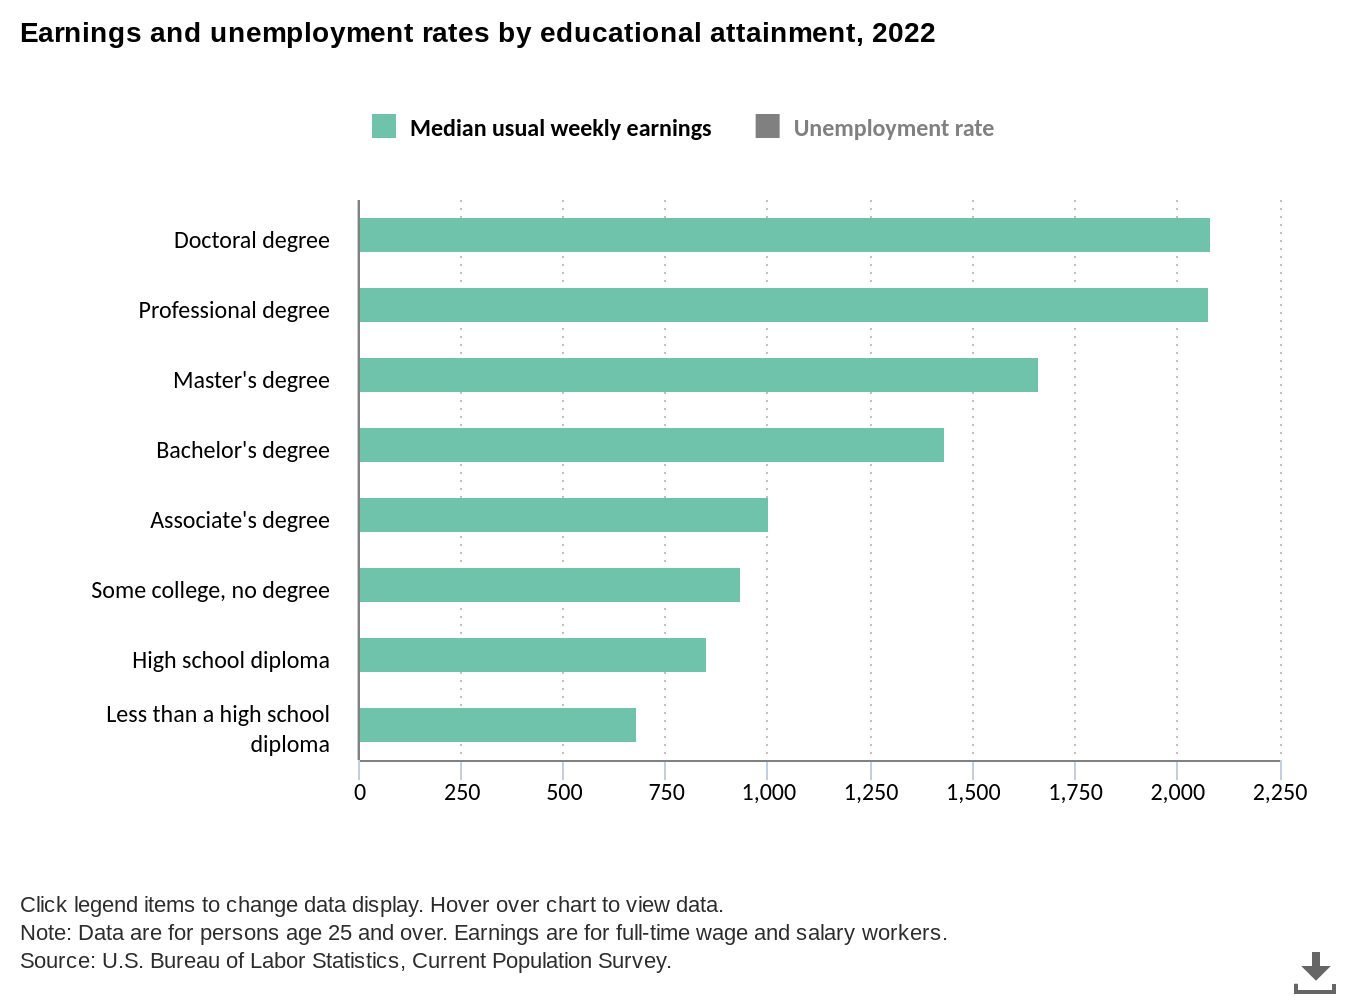
\includegraphics[width=0.9\textwidth]{pictures/earnings-and-unemploymen.png}
    Source: Bureau of Labor Statistics, ``Education Pays, 2022"
\end{frame}

\begin{frame}{Why Are More Educated People Paid More?}
    \begin{wideitemize}

        \item Selection: People who are more productive tend to get an education
        \begin{wideitemize}
            \item Education is not making them productive.
            \item Rather, it signals that they are already productive.
        \end{wideitemize}
        \item Treatment: Education makes people more productive.

    \end{wideitemize}
\end{frame}


\begin{frame}{The Returns to Education}

\begin{wideitemize}
    \item Econometrically, we can say that a person's income can be decomposed as:
\[\underbrace{I}_{\text{income}}  = \beta \cdot \underbrace{E}_{\text{education}} + \underbrace{a}_{\text{latent productivity}}\]
\item $\beta$ is the return to education, and it is important for policymakers.
\item Discussion: Why?
\item You cannot typically just regress income on education, because education is correlated with latent productivity.
\item This is exactly the selection effect we talked about on the last slide.
\item There is an entire literature trying to estimate the returns to education ($\beta$).
\end{wideitemize}
\end{frame}

\begin{frame}{But Wait...}

\begin{wideitemize}
    \item This class is about compensation within organizations.
    \item It is not about setting education policy. So what do we care about?
    \item Organizations care about hiring productive people.
    \item Whether education made them productive or they were productive prior to being educated is not the main concern.
    \item It can be a big concern if an organization pays members to go to school.
    \item Then knowing the return to education matters, because the org. is encouraging education directly.
\end{wideitemize}
\end{frame}


\section{Signaling Role of Education}

\begin{frame}{Removing the Return to Education}

\begin{wideitemize}
    \item It is relatively straightforward to think about how the returns to education works.
    \item If I learn to read, I can receive and follow directions.
    \item If I learn to prepare a centrifuge, I can work in certain types of labs.
    \item But suppose the return to education is 0.
    \item Does it still make sense for an organization to pay higher wages to more educated people?
    \item Thinking through this question also helps us ask when an organization should ever pay people based on an observable characteristic.
\end{wideitemize}
    
\end{frame}

\begin{frame}{Model (Job Market Signaling)}

\begin{wideitemize}
    \item There is a single worker and two firms
    \item Worker is either high productivity ($t=H$) with prob. $p$ or low productivity ($t=L$) with prob. $1-p$.
    \item Profit from hiring low-skill is 0 and high-skill is $\pi>0$
    \item First, the worker can acquire education $E=1$ at cost $c_t$ where $c_H<c_L$ (Why?) or not ($E=0$) at cost 0.
    \item  After observing education each firm posts a wage Bertrand style.
    \item After observing the wage, the worker chooses a firm. Assume the worker flips a coin when indifferent.
\end{wideitemize}
\end{frame}


\begin{frame}{Model: Important Feature}
\begin{wideitemize}
    \item Importantly firms do not observe productivity.
    \item They do know the probability the person is high or low productivity.
    \item This is equivalent to knowing the fraction of the population that is each type.
    \item They also see education.
    \item We need to understand how beliefs change when a firm sees a high education person.
\end{wideitemize}
    
\end{frame}

% \begin{frame}{A Helpful Tool: Bayes' Rule}

% \begin{wideitemize}
%     \item In order to understand how a belief should be updated based on new information (education choice) we need Bayes' Rule.
    
%     \begin{theorem}
%     Given two events A and B Bayes' Rule states that:
%     \[Pr(A | B) = \frac{Pr(A \& B)}{Pr(B)} = \frac{Pr(B | A)Pr(A)}{Pr(B)} \]
%     \end{theorem}
%     \item $Pr(A|B)$ reads the probability of A given B.
%     \item Generally $A$ is the type of other player, and $B$ is some action taken by other player.
%     \item In equilibrium, sometimes different types play different strategies which makes the actions a signal.
% \end{wideitemize}
    
% \end{frame}
\begin{frame}{Solving the Model}
\Huge See the Board!
    
\end{frame}

\begin{frame}{Solution}

\begin{theorem}
    The following are equilibrium outcomes under the assumption that $c_H<\pi < c_L$:
    \begin{wideitemize}
        \item Only high productivity workers get an education
        \item No one gets an education, and firms believe those with an education have the same probability of being high productivity than those without.
        \item Everyone gets an education, and firms believe those without an education are low productivity.
    \end{wideitemize}
\end{theorem}
    \begin{wideitemize}
        \item It is clear that education can serve as a signal of productivity.
        \item This is true even when the return to education is 0.
    \end{wideitemize}
\end{frame}

\begin{frame}{Beliefs are Self-Confirming}

\begin{wideitemize}
    \item If firms believe educated people are productive, education becomes valuable.
    \item If firms believe educated people are no different than non-educated, education is worthless.
\end{wideitemize}
    
\end{frame}

\begin{frame}{Education as a Costly Signal}

\begin{wideitemize}
    \item Notice that we needed the assumption that $c_H<\pi < c_L$
    \item The opportunity cost of education for high productivity people must be much less than for low productivity people.
    \item Discussion: Is this true?
    \item This is necessary for education (or anything) to be a signal.
    \item Analogy: advertising
    \item It allows productive people to separate themselves, because it is too costly for low productivity people to follow.
    \item As we discussed, it is not sufficient (we also need the right beliefs!)
\end{wideitemize}
    
\end{frame}

\section{How Much Is Signaling vs. Returns to Education?}


\begin{frame}{Aryal et. al. (2022)}
    \begin{wideitemize}
        \item The authors call the total effect of education on wage the ``private return."
        \item In our language this is the signaling effect plus the returns to education.
        \begin{wideitemize}
            \item Key idea: if something shifts education that employers do not observe, we can uncover the private return!
            \item Discussion: why?
        \end{wideitemize}
        \item They call the returns to education (the direct productivity increase) the ``social return."
         \begin{wideitemize}
            \item Key idea: if something shifts education that employers do observe, we can uncover the social return!
            \item Discussion: why?
        \end{wideitemize}
    \end{wideitemize}
\end{frame}
\begin{frame}{A Natural Experiment}
    \begin{wideitemize}
       \item Norway extended compulsory schooling from 7 to 9 years between 1960 and 1975.
       \item Crucially, it rolled out the program across the country slowly.
       \item Jobs are concentrated in the central cities, but workers come from across the country.
       \item For example, Oslo implemented the law in 1967 but surrounding areas implemented it as early as 1961 and as late as 1971.
       \item If you grew up in a central city, employers likely understood how the law impacted your schooling decisions.
       \item If you grew up in one of the many outlying regions, they likely did not.
    \end{wideitemize}
\end{frame}

\begin{frame}{A Natural Experiment}
    \begin{wideitemize}
       \item We can analyze how the reform impacted wages of those who grew up in central regions to get the social return.
       \item We can analyze how the reform impacted wages of those who grew up in non-central regions to get the private return.
       \item Norway also has mandatory military service and thus administers an IQ test to males.
       \item So we can ask whether education could be a signal.
    \end{wideitemize}
\end{frame}


\begin{frame}{Should We Expect Signaling?}
\centering
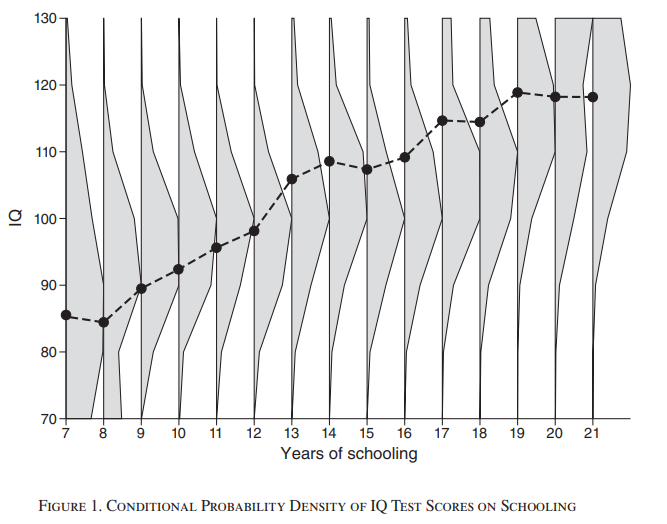
\includegraphics[width=0.7\textwidth]{pictures/iq_norway.png}
\end{frame}

\begin{frame}{Did the Law Increase Schooling?}
\centering
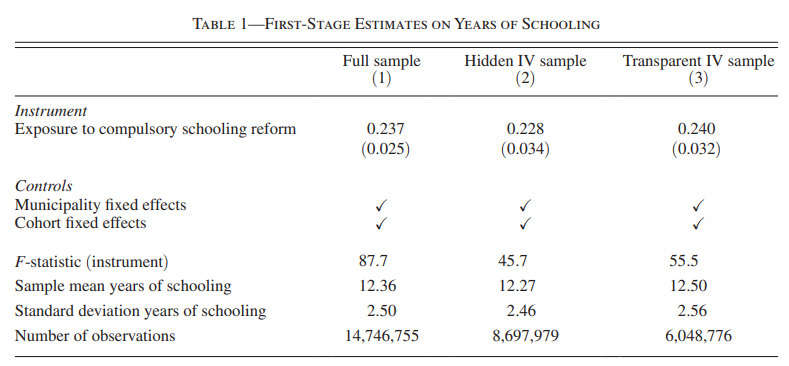
\includegraphics[width=0.85\textwidth]{pictures/norway_increase.png}
\end{frame}

\begin{frame}{Did The Law Increase Wages?}
\centering
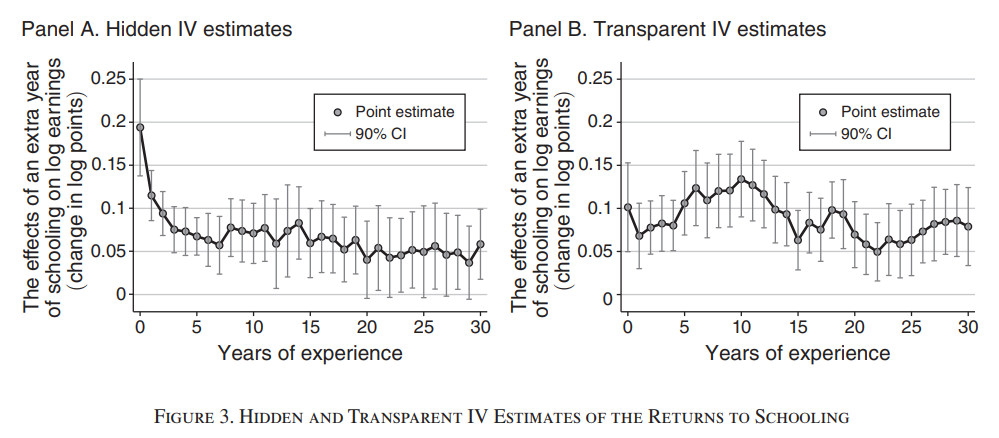
\includegraphics[width=0.95\textwidth]{pictures/wages_norway.png}
\end{frame}

\begin{frame}{Signaling and the Private Returns to Education}

\begin{wideitemize}
    \item The initial private return is 19.8 percent.
    \item But this value decreases rapidly to 5.5 percent as a worker is employed.
    \item Employers put only a 16.4 percent weight on the initial education signal from workers.
    \item Confirms an old adage: your degree matters most for your first job, then your first job matters.
\end{wideitemize}
    
\end{frame}
\begin{frame}{The Returns to Education (Social Return)}

\begin{wideitemize}
    \item The social return is estimated to be 5.5 percent.
    \item The private return converges to the social return as signaling vanishes!
    \item Bottom-line: the authors estimate that of the total wage return to education, 70 percent is a productivity increase from education while 30 percent is signaling.
\end{wideitemize}
    
\end{frame}

\end{document}




